\chapter{Wykorzystane technologie (AK i~JC)}
\label{ch:technologies}

% setup
\graphicspath{{2_technologies/static/}}

% content
W~niniejszym rozdziale zawarty został opis stosowanych przez autorów pracy technologii. Przedstawione informacje obejmują zarówno wykorzystane języki programowania, jak również narzędzia, których zadaniem jest ułatwienie tworzenia wysokiej jakości kodu źródłowego, czy też automatyzacja procesów zachodzących na różnych etapach cyklu życia oprogramowania. Niniejszy rozdział stanowi krótkie wprowadzenie do każdego z~omawianych zagadnień - zaawansowane aspekty każdej z~opisywanych technologii przedstawione zostały w~dalszej części pracy, podczas omawiania konkretnych, osiągniętych za ich pomocą, rozwiązań. 


\section{Język C++ (AK)}
C++ \cite{Bjarne} \cite{cpp_reference} to stworzony w~latach 80-tych XX wieku wszechstronny język programowania, oryginalnie mający stanowić rozszerzenie popularnego języka C~\cite{c_book} o~mechanizmy pozwalające na programowania obiektowe. Wraz z~jego rozwojem pojawiło się natomiast wsparcie dla innych paradygmatów programowania, dzięki czemu nowoczesny C++ pozwala stosować (poza paradygmatem proceduralnym oraz obiektowym) programowanie funkcyjne oraz generyczne. Z~tego też powodu język ten znajduje współcześnie bardzo szerokie zastosowanie, od rozwiązań telekomunikacyjnych po oprogramowanie dla eksperymentów fizycznych, takich jak detektor ATLAS w~CERN. Jest on ponadto bardzo istotny z~punktu widzenia niniejszej pracy, ponieważ za jego pomocą napisana została większość oprogramowania systemu GGSS.

C++ jest wydajnym językiem kompilowanym, opartym o~statyczne typowanie. Udostępnia mechanizmy pozwalające programiście na działanie na wielu poziomach abstrakcji - możliwe są zarówno niskopoziomowe operacje, takie jak manualne zarządzanie pamięcią, jak również modelowanie wysokopoziomowej logiki biznesowej. W~ciągu ostatnich dziesięciu lat miał miejsce szczególnie intensywny rozwój języka, czego początek stanowi pojawienie się przełomowego standardu C++11. Od tego czasu regularnie, co trzy lata, wydawana jest nowa wersja standardu języka, a~zatem od 2011 roku pojawiły się następujące wydania:
\begin{itemize}
\item C++11 - uznawane za przełomowe, zawiera modyfikacje w~znacznym stopniu zmieniające sposób tworzenia oprogramowania w~języku C++. Wprowadzone zostały zarówno rozszerzenia w~rdzeniu języka, jak i~w bibliotece standardowej. Najważniejsze elementy standardu C++11 to m.in.: semantyka przenoszenia i~referencje do \emph{r-wartości}, wyrażenia lambda, słowa kluczowe \lstinline{override} i~\lstinline{final} ułatwiające programowanie obiektowe, inferencja typów za pomocą słowa kluczowego \lstinline{auto}, wsparcie dla wielowątkowości (model pamięci oraz funkcjonalności w~bibliotece standardowej), tzw. inteligentne wskaźniki (ang. \emph{smart pointers}) ułatwiające zarządzanie pamięcią czy nowe kontenery biblioteki standardowej.
\item C++14 - mniejsze wydanie, stanowiące uzupełnienie standardu C++11 o~pomniejsze funkcjonalności oraz poprawki. Wprowadzone zmiany to m.in. ułatwienia w~korzystaniu ze słowa kluczowego \lstinline{constexpr} oraz generyczne wyrażenia lambda. 
\item C++17 - wprowadza wiele nowych funkcjonalności, m.in. bibliotekę do obsługi systemu plików, typ \lstinline{std::optional} czy możliwość wykonania inicjalizacji w~wyrażeniu warunkowym \cite{cpp17_book}.
\item C++20 - najnowsze wydanie języka, pod względem liczby wprowadzonych zmian większe od dwóch poprzednich. Przykładowe elementy tego standardu to: koncepty (ang. \emph{concepts}), moduły czy biblioteka pozwalająca na operacje na zakresach (ang. \emph{ranges}).
\end{itemize}

Obecnie trwają pracę nad nowym standardem języka, którego publikacja planowana jest na rok 2023. Poza wprowadzaniem funkcjonalności, nowe wydania języka C++ eliminują te elementy języka, które uznawane są za przestarzałe. Przykładem może być obecny w~bibliotece standardowej od wczesnych wersji języka inteligentny wskaźnik \lstinline{std::auto_ptr} - został on oznaczony jako przestarzały (ang. \emph{deprecated}) po pojawieniu się nowych rozwiązań w~standardzie C++11, a~następnie został usunięty z~języka wraz z~wprowadzeniem standardu C++17. Tego typu zmiany mają na celu wspieranie tzw. \emph{dobrych praktyk} - zasad ułatwiających tworzenie łatwego w~utrzymaniu i~rozwoju oprogramowania (np. poprzez odpowiednie zarządzanie zasobami).

Z~punktu widzenia niniejszej pracy szczególnie istotne są zmiany wprowadzone w~standardzie C++11 - z~uwagi na ograniczenia w~środowisku docelowym systemu GGSS jest to najnowsze dostępne tam wydanie języka (więcej informacji na ten temat przedstawione zostało w~dalszej części pracy). Dlatego też zaprezentowany został krótki przykład obrazujący część funkcjonalności wprowadzonych właśnie w~tym standardzie. W~przykładzie tym zaimplementowana została prosta hierarchia klas reprezentujących zasilacze: jedna abstrakcyjna klasa bazowa \lstinline{PowerSupply} oraz dwie implementacje: \lstinline{CaenPowerSupply} oraz \lstinline{MockPowerSupply}. W~funkcji \lstinline{main()} tworzony i~wypełniany jest kontener przechowujący wskaźniki zawierające adresy obiektów reprezentujących różne typy zasilaczy. Następnie dla każdego z~istniejących zasilaczy następuje polimorficzne wywołanie metody pozwalającej na zmianę wartości zasilania (tutaj powoduje jedynie wypisanie odpowiedniej wiadomości na standardowe wyjście). Celem przykładu jest zaprezentowanie prostego scenariusza, w~którym nowe funkcjonalności języka wpływają pozytywnie na jakość i~bezpieczeństwo kodu - nie prezentuje więc on w~sposób bezpośredni zaawansowanych elementów języka (takich jak możliwość metaprogramowania za pomocą szablonów).

Na listingu \ref{lst:cpp_old} przedstawiona została implementacja przykładu zgodna ze standardem C++03. Najważniejsze cechy zaprezentowanego kodu, charakterystyczne dla kodu źródłowego powstającego przed pojawieniem się standardu C++11, to: 
\begin{itemize}
\item konieczność manualnego zarządzania pamięcią - widoczne zastosowanie operatora \lstinline{delete} pod koniec funkcji \lstinline{main()}
\item brak bezpośredniej możliwości zadeklarowania klasy jako \emph{finalna} - tzn. taka, po której nie można dziedziczyć (przed standardem C++11 istniały jednak techniki, wykorzystujące zaawansowane funkcjonalności języka, pozwalające osiągnąć podobny rezultat - ze względu na stopień skomplikowania nie zostały tu jednak zaprezentowane)
\item brak możliwości wskazania, że metoda w~klasie pochodnej nadpisuje (ang. \emph{override}) metodę wirtualną z~klasy bazowej
\item rozbudowana, nieczytelna składnia pętli \lstinline{for} operującej na kontenerze za pomocą iteratora 
\end{itemize}

\lstinputlisting[
    language=C++, 
    caption={Przykładowa implementacja prostej hierarchii dziedziczenia oraz polimorficznego wykonania metody - standard C++03. Należy zwrócić uwagę na konieczność manualnego zarządzania pamięcią oraz brak możliwości wskazania, że metoda w~klasie pochodnej nadpisuje metodę wirtualną z~klasy bazowej.}, 
    label={lst:cpp_old}
]{2_technologies/code_samples/cpp_example_old.cpp}


Na listingu \ref{lst:cpp_new} przedstawiona została natomiast implementacja przykładu za pomocą języka C++ w~standardzie 11. Najważniejszą zmianą jest zastosowanie inteligentnego wskaźnika \lstinline{std::unique_ptr<PowerSupply>}, automatyzującego zarządzanie wskazywanym zasobem (pamięć zostaje zwolniona, gdy wskaźnik ulega destrukcji). Powoduje to, że programista nie jest odpowiedzialny za manualne sprawowanie kontroli nad pamięcią, a~co za tym idzie zmniejsza prawdopodobieństwo wystąpienia związanych z~tym błędów (takich jak wycieki pamięci). Kolejną zmianą jest zastosowanie słowa kluczowego \lstinline{override} w~celu zadeklarowania, że metoda w~klasie pochodnej (np. \lstinline{CaenPowerSupply}) nadpisuje metodę z~klasy bazowej (tutaj \lstinline{PowerSupply}). W~przypadku, gdy powyższe nie jest prawdą (np. za sprawą błędnej pisowni lub braku słowa kluczowego \lstinline{const}), kompilator zgłosi błąd. W~klasach pochodnych zastosowane zostało ponadto słowo kluczowe \lstinline{final}, powodujące, że po klasach tych nie można dziedziczyć - jego stosowanie może wynikać m.in. z~zalecenia mówiącego, że dziedziczenie powinno być możliwe jedynie w~przypadku klas, które są z~myślą o~nim projektowane (np. klasy abstrakcyjne). Wymienione powyżej zmiany, możliwe dzięki stosowaniu funkcjonalności nowoczesnego języka C++, pozwalają na zwiększenie niezawodności tworzonego kodu źródłowego, m.in. poprzez zabezpieczenie go przed prostymi błędami oraz dostarczenie dodatkowej, wbudowanej wprost w~język, dokumentacji. Innym typem zmiany, nastawionym w~większym stopniu na zwiększenie czytelności kodu, jest natomiast zastosowanie w~przykładzie pętli zakresowej do iteracji po kontenerze oraz wykorzystanie słowa kluczowego \lstinline{default} w~deklaracji domyślnego destruktora wirtualnego klasy bazowej. W~standardzie C++11 wprowadzonych zostało znacznie więcej podobnych udoskonaleń, a~ponadto wprowadzone zostały mechanizmy ułatwiające optymalizację oprogramowania (np. ze względu na szybkość wykonania lub ilość zużytej pamięci) - jednak ze względu na konieczność zachowania prostego charakteru przykładu nie zostały one zaprezentowane.

\lstinputlisting[
    language=C++, 
    caption={Przykładowa implementacja prostej hierarchii dziedziczenia oraz polimorficznego wykonania metody - standard C++11. Widoczne zastosowanie słów kluczowych \lstinline{default}, \lstinline{final} oraz \lstinline{override}, pętli zakresowej oraz inteligentnego wskaźnika.}, 
    label={lst:cpp_new}
]{2_technologies/code_samples/cpp_example_new.cpp}

\clearpage
Język C++ charakteryzuje się ponadto istnieniem dodatkowych, nie będących częścią standardu, bibliotek poszerzających zestaw dostarczanych przez niego narzędzi. Z~punktu widzenia systemu GGSS istotne są: zestaw bibliotek Boost \cite{Boost_main} \cite{Boost_docs}, biblioteka GNU Scientific Library (GSL) \cite{GSL_main} oraz zestaw bibliotek i~narzędzi Qt \cite{Qt_main}.

Boost to popularna kolekcja bibliotek dla języka C++, ułatwiająca wiele aspektów tworzenia oprogramowania poprzez dostarczenie zróżnicowanego zestawu narzędzi programistycznych: zarówno ogólnego przeznaczenia, jak i~bardzo wyspecjalizowanych. Pakiet Boost rozwijany jest znacznie szybciej niż biblioteka standardowa języka C++, a~ponadto niektóre jego elementy stanowiły podstawę dla funkcjonalności dodawanych do języka w~nowych jego wydaniach (np. wprowadzona w~standardzie C++17 biblioteka \lstinline{filesystem}, służąca do zarządzania systemem plików, oparta jest na analogicznym module z~zestawu Boost). Przykładowe funkcjonalności udostępniane przez pakiet Boost to: rozszerzona względem biblioteki standardowej obsługa łańcuchów znakowych, dodatkowe kontenery (np. \lstinline{Boost.MultiIndex}), implementacja algorytmów grafowych czy asynchroniczne programowanie sieciowe. Ze względu na szeroki zakres oferowanych funkcjonalności, pakiet Boost stosowany jest również przez warstwę oprogramowania omawianego w~niniejszej pracy systemu GGSS.

GNU Scientific Library (GSL) to napisana w~języku C~biblioteka udostępniająca narzędzia programistyczne do wykonywania obliczeń numerycznych. Pozwala na wykonywanie operacji takich jak: znajdowanie miejsc zerowych funkcji, dopasowywanie krzywej do danych czy całkowanie metodą Monte Carlo \cite{MC_wikipedia}. Ze względu na drugą z~wymienionych tu funkcjonalności biblioteka ta znalazła zastosowanie w~oprogramowaniu systemu GGSS.

Qt jest zestawem narzędzi programistycznych umożliwiających tworzenie przenośnych aplikacji okienkowych z~wykorzystaniem języka C++. Technologia ta nie została zastosowana w~rdzeniu oprogramowania systemu GGSS, natomiast przy jej pomocy stworzone zostały pomniejsze narzędzia wchodzące w~skład projektu. Opisane w~niniejszej pracy rozwiązania nie są oparte o~Qt, dlatego też szczegółowy opis dostarczanych przez zestaw narzędzi nie zostanie w~niej zamieszczony.


\section{Język Python (AK)}
Python \cite{Python_main} \cite{Lutz} jest opartym na dynamicznym systemie typów językiem programowania ogólnego przeznaczenia, charakteryzującym się bardzo szerokim obszarem zastosowań, obejmującym m.in. automatyzację za pomocą skryptów, tworzenie aplikacji internetowych czy eksplorację danych. Cechą najczęściej kojarzoną z~tym językiem jest intuicyjna składnia, ułatwiająca zarówno jego naukę, jak i~zrozumienie napisanych z~jego pomocą programów. Python jest językiem wieloparadygmatowym, pozwalającym pisać zarówno w~sposób proceduralny, jak i~obiektowo i~funkcyjnie. W~systemie GGSS język ten stosowany jest jako narzędzie pomocnicze, rozumiane przede wszystkim jako język skryptowy wykorzystywany do tworzenia infrastruktury projektu.

Obecnie język Python istnieje w~dwóch szeroko stosowanych wersjach: Python 2~oraz Python 3. Oficjalnie wspieraną wersją jest wydanie trzecie (wsparcie dla Pythona w~wersji drugiej zakończone zostało na początku 2020 roku), w~rzeczywistości jednak, ze względu na fakt, iż wersje te nie są ze sobą w~pełni kompatybilne, oprogramowanie napisane za pomocą Pythona 2~wciąż znaleźć można w~wielu projektach. Z~punktu widzenia systemu GGSS różnice między tymi wydaniami nie są w~dużym stopniu znaczące (ponieważ język ten używany jest jako pomocnicze narzędzie), jednakże preferowana jest wersja trzecia.

Na listingu \ref{lst:python} przedstawiony został prosty przykład zastosowania języka Python jako narzędzia do tworzenia skryptów. W~tym przypadku jest to prosty skrypt, generujący sto pierwszych elementów ciągu Fibonacciego i~zapisujący je do pliku tekstowego w~postaci kolumny. Przykład obrazuje wykorzystanie takich elementów języka jak generatory, pętle oraz operacje na plikach.


\lstinputlisting[
    language=Python, 
    caption={Przykładowy skrypt napisany w~języku Python, którego działanie polega na wygenerowaniu stu pierwszych elementów ciągu Fibonacciego i~zapisaniu otrzymanego wyniku do pliku tekstowego.}, 
    label={lst:python}
]{2_technologies/code_samples/python_example.py}


\section{Narzędzia do analizy oprogramowania (AK)}
Podczas prac nad systemem GGSS autorzy wykorzystali szereg narzędzi ułatwiających utrzymanie jakości oraz niezawodności tworzonego oprogramowania. Współcześnie, wraz z~rosnącym skomplikowaniem powstających projektów informatycznych, rośnie zapotrzebowanie na narzędzia wspierające analizę tworzonego oraz rozwijanego oprogramowania - jest ono często utrzymywane przez wiele osób, przez co zachowanie jego wysokiej jakości staje się coraz bardziej wymagającym zadaniem. Opisywane narzędzia charakteryzują się szerokim zakresem oferowanych możliwości, m.in. monitorowanie zużycia zasobów czy też badanie kodu źródłowego pod kątem zgodności z~pewnymi przyjętymi standardami, oraz wspierają wykonywanie analizy programu na wiele zróżnicowanych sposobów. W~najprostszym ujęciu wskazać można dwie możliwości klasyfikacji technik analizy oprogramowania:
\begin{itemize}
    \item analiza kodu źródłowego (ang. \emph{source analysis}) oraz analiza kodu maszynowego (ang. \emph{binary analysis}) - w~przypadku pierwszego typu badaniom poddawany jest kod źródłowy, napisany np. z~wykorzystaniem języka C++, drugie podejście polega natomiast na analizie programu na poziomie kodu maszynowego lub reprezentacji pośredniej, takiej jak kod bajtowy (ang. \emph{bytecode}).
    \item analiza statyczna (ang. \emph{static analysis}) oraz analiza dynamiczna (ang. \emph{dynamic analysis}) - podejścia te różni to, czy badanie wykonywane jest bez uruchamiania programu (pierwszy typ), czy też w~trakcie jego wykonywania (drugi rodzaj).
\end{itemize}

Powyższe dwa podziały pozwalają ostatecznie określić cztery kategorie analizy oprogramowania: statyczna analiza kodu źródłowego, statyczna analiza kodu maszynowego, dynamiczna analiza kodu źródłowego oraz dynamiczna analiza kodu maszynowego \cite{code_analysis}. Każde z~tych podejść charakteryzuje się pewnymi zaletami względem pozostałych, należy je jednak traktować jako komplementarne - wskazane jest, w~zależności od potrzeb, wykorzystywanie różnego typu narzędzi ułatwiających utrzymanie wysokiej jakości tworzonego oprogramowania. Szczegółowa analiza każdej z~wymienionych możliwości wykracza poza zakres niniejszej pracy, w~dalszej jej części przedstawione zostały jedynie najważniejsze informację na temat szczególnie istotnych narzędzi, które wykorzystywali autorzy podczas prac nad systemem GGSS. W~zamieszczonym opisie pominięte zostało jednak oprogramowanie, którego znajomość nie jest konieczna w~celu zrozumienia dalszych części niniejszego manuskryptu, takie jak GNU Debugger (GDB) \cite{gdb}.

Z~punktu widzenia testów, jakie wykonywane były podczas prac nad systemem GGSS, bardzo istotna jest platforma Valgrind \cite{valgrind}. Jej działanie opiera się na przeprowadzaniu tzw. instrumentacji - umieszczaniu w~kodzie dodatkowych instrukcji \cite{reverse}, pozwalających na wykonywanie jego analizy, co w~tym przypadku ma miejsce w~czasie wykonywania programu. Valgrind pozwala na tworzenie wyspecjalizowanych narzędzi wykorzystujących dynamiczną instrumentację binarną, dzięki udostępnieniu rdzenia (ang. \emph{core}), którego zadaniem jest deasemblacja kodu maszynowego do tzw. postaci pośredniej. Postać ta wykorzystywana jest przez poszczególne narzędzia, które dodają odpowiedni dla danego zastosowania kod analizujący. Szczególnie istotne z~punktu widzenia niniejszej pracy są narzędzia Memcheck \cite{memcheck_1} \cite{memcheck_2} oraz Massif \cite{massif}, których zadaniem jest monitorowanie, w~jaki sposób badany program wykorzystuje dostępną pamięć.

Memcheck jest domyślnym narzędziem udostępnianym przez platformę Valgrind, pozwalającym na wykrywanie błędów związanych z~zarządzaniem pamięcią w~programach napisanych w~językach C~i C++. Przykładem tego typu błędów są wycieki pamięci, użycie zmiennych, którym nie została nadana żadna wartość, oraz próby dostępu do zwolnionej pamięci. Memcheck jest szczególnie istotny w~kontekście testów systemu GGSS, ponieważ pozwala upewnić się, że podczas działania aplikacji wchodzących w~skład projektu nie mają miejsca żadne błędy mogące powodować stopniowy wzrost zużycia zasobów, co w~przypadku systemu działającego nieprzerwanie przez wiele miesięcy jako usługa mogłoby doprowadzić do niespodziewanej awarii. 

Na listingu \ref{lst:memcheckcode} przedstawiony został fragment kodu źródłowego napisanego w~języku C++, zawierającego przykłady prostych błędów, które mogą zostać wykryte przy użyciu narzędzia Memcheck: użycie niezainicjalizowanej zmiennej oraz wyciek pamięci. W~funkcji \lstinline{main()} tworzona jest zmienna \lstinline{no_value}, której nie zostaje nadana wartość. Następnie na jej podstawie podejmowana jest decyzja o~zmianie wartości zmiennej \lstinline{value} - sprawia to, że działanie programu jest niemożliwe do przewidzenia. W~ostatniej linii funkcji \lstinline{main()} tworzona jest dynamiczna tablica dziesięciu liczb całkowitych - ponieważ w~programie nie następuje jej zwolnienie, jest to prosta forma wycieku pamięci.

\lstinputlisting[
    language=C++, 
    caption={Przykład prostego programu zawierającego błędu możliwe do wykrycia za pomocą narzędzia Memcheck: użycie zmiennej, której nie została nadana wartość oraz wyciek pamięci.}, 
    label={lst:memcheckcode}
]{2_technologies/code_samples/memcheck_code.cpp}

Na listingu \ref{lst:memcheckcmd} przedstawione zostało natomiast wywołanie narzędzia Memcheck w~celu zbadania stanowiącego przykład programu. W~zamieszczonym wyjściu widoczne są informacje na temat wykrycia obu błędów. Ponadto, ponieważ nastąpiło wywołanie z~użyciem opcji \lstinline{--track-origins=yes}, wskazywane jest źródło wystąpienia nieprawidłowości (np. w~przypadku niezainicjalizowanej zmiennej jest to linia, w~której następuje jej definicja). Ponadto wyświetlane są: podsumowanie zawierające informacje na temat dynamicznych alokacji pamięci (czyli na tzw. stercie - ang. \emph{heap}) oraz raport podsumowujący wykryte przez narzędzie wycieki pamięci, w~zależności od ich rodzaju.

\lstinputlisting[
    language=Cmd, 
    caption={Wywołanie narzędzia Memcheck w~celu zbadania programu zamieszczonego na listingu \ref{lst:memcheckcode} - widoczne informacje na temat obu obecnych w~przykładzie błędów.}, 
    label={lst:memcheckcmd}
]{2_technologies/code_samples/memcheck_output.txt}

W~niniejszej pracy pominięty został szczegółowy opis technik stosowanych przez narzędzie Memcheck w~celu wykrywania błędów występujących w~badanym programie. Istotna jest natomiast informacja, że przeprowadzana analiza oparta jest na wykorzystywaniu dodatkowych zasobów, w~tym znaczącej ilości pamięci. W~ten sposób działa m.in. mechanizm wykrywania użycia niezainicjalizowanych zmiennych - każdy bit danych zarządzany przez badany proces jest śledzony przez narzędzie za pomocą metadanych w~postaci innego bitu (tzw. \emph{valid-value bit}) \cite{memcheck_1}. Powoduje to znaczący wzrost zużycia pamięci, a~zatem uniemożliwia jednoczesne przeprowadzanie (np. za pomocą innych, zewnętrznych narzędzi) badań dotyczących ilości wykorzystywanych przez analizowany program zasobów.

Drugim, istotnym z~uwagi na prezentowane w~niniejszym manuskrypcie treści, narzędziem opartym o~platformę Valgrind jest Massif. Umożliwia on generowanie szczegółowych raportów opisujących wykorzystanie pamięci sterty (oraz opcjonalnie stosu) przez badany program. Pozwala to wykrywać scenariusze takie jak stopniowo rosnący, wraz z~długotrwałym działaniem programu, rozmiar dynamicznie alokowanych struktur danych. Ponieważ w~takim przypadku wyciek pamięci nie następuje w~sposób jawny, problem tego typu jest trudny do wykrycia za pomocą narzędzia Memcheck. Uproszczony przykład tego typu scenariusza przedstawiony został na listingu \ref{lst:massif_code}. Zamieszczony tam program symuluje sterowany przez użytkownika pomiar: w~każdej iteracji pętli \lstinline{do-while} następuje alokacja pamięci, a~następnie na podstawie wprowadzonego na standardowe wejście znaku podejmowana jest decyzja o~kontynuacji lub zakończeniu działania. Po zakończeniu wykonywania pętli następuje zwolnienie pamięci. Przedstawiony program nie zawiera błędów związanych z~zarządzaniem pamięciom - zastosowania narzędzia Memcheck nie wskazuje na występowanie żadnych problemów. Każda iteracja pętli \lstinline{do-while} wiąże się jednak ze zwiększeniem rozmiaru wykorzystywanej przez program pamięci sterty, co ostatecznie może doprowadzić do jej wyczerpania, a~co za tym idzie, do błędu kończącego działanie aplikacji. Tego typu scenariusz jest szczególnie niebezpieczny w~przypadku aplikacji, od których oczekuje się bezawaryjnego działania przez bardzo długi czas (np. kilka miesięcy) - w~tego typu przypadkach mechanizm sterujący alokacją pamięci może być znacząco bardziej skomplikowany, niż ten przedstawiony w~przykładzie, a~co za tym idzie wczesne wykrycie potencjalnego problemu może być niemożliwe bez zastosowania narzędzia takiego jak Massif.

\lstinputlisting[
    language=C++, 
    caption={Przykład prostego programu symulującego cykliczne wykonywanie pomiaru. W~każdej iteracji wykonywana jest dynamiczna alokacja pamięci, a~użytkownik za pomocą standardowego wejścia decyduje o~zaprzestaniu lub kontynuacji działania programu. Załączony kod obrazować ma sytuację, w~której program stopniowo zwiększa zużycie dostępnych zasobów, co w~konsekwencji doprowadzić może do przerwania jego działania, gdy zostaną one wyczerpane.}, 
    label={lst:massif_code}
]{2_technologies/code_samples/massif_code.cpp}

Na rysunku \ref{fig:massif_plot} przedstawiony został natomiast wykres wykonany za pomocą danych, jakie znalazły się w~raporcie wygenerowanym przez narzędzie Massif. Przedstawia on zużycie pamięci sterty w~funkcji czasu dla przykładowego uruchomienia zaprezentowanego programu - wyraźnie widoczny jest wzrost ilości wykorzystywanych zasobów wraz z~kolejnymi alokacjami następującymi w~pętli \lstinline{do-while}. Poza danymi liczbowymi na temat zużycia przez badany program pamięci, generowany przez narzędzie raport zawiera informacje na temat następujących alokacji, co ułatwia znajdowanie źródeł wzrostu wykorzystania zasobów. Ze względu na znaczny rozmiar generowanego raportu nie został on zaprezentowany w~niniejszym manuskrypcie.

\begin{figure}[H]
\centering
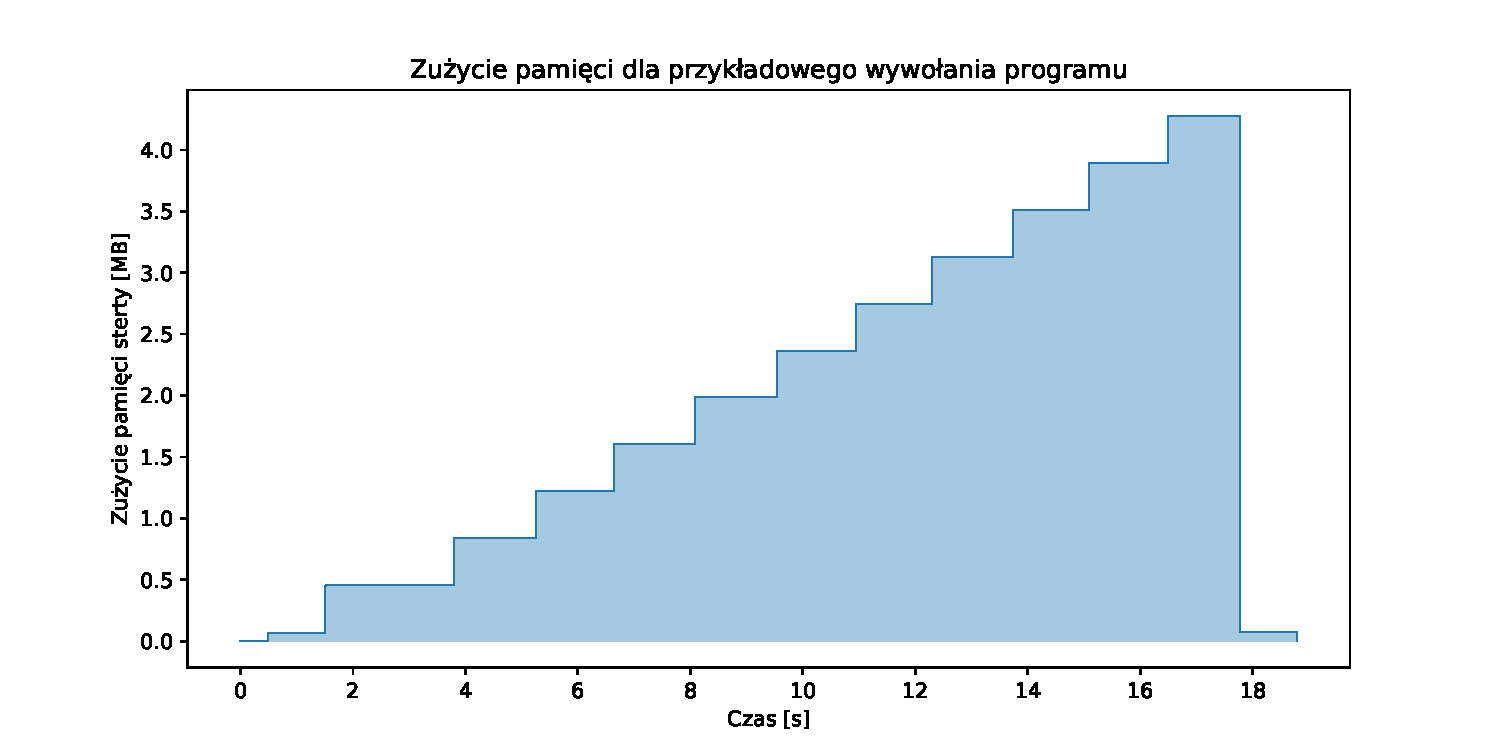
\includegraphics[width=\textwidth]{massif_plot.pdf}
\caption{Wykres przedstawiający ilość wykorzystywanej pamięci sterty w~funkcji czasu. Zaprezentowane dane pochodzą z~przykładowego uruchomienia programu zawartego na listingu \ref{lst:massif_code} - ich pozyskanie możliwe było dzięki wykorzystaniu wygenerowanego przez narzędzie Massif raportu.}
\label{fig:massif_plot}
\end{figure}

Innym typem narzędzi wykorzystywanych przez autorów niniejszej pracy są te służące do statycznej analizy kodu źródłowego w~celu określenia jego zgodności z~przyjętymi konwencjami. Wykonywane w~ten sposób badanie pozwala wykryć nieprawidłowości związane zarówno z~tak prostymi zagadnieniami jak przyjęty styl (np. nazewnictwo zmiennych czy kolejność załączania plików nagłówkowych), jak również z~wykorzystaniem poszczególnych elementów języka programowania (np. wykrywanie przestarzałych, niezalecanych konstrukcji, takich jak wspomniany w~części opisującej język C++ wskaźnik \lstinline{std::auto_ptr}). Tego typu narzędzia w~znaczącym stopniu ułatwiają refaktoryzację (ang. \emph{refactoring}), czyli proces wprowadzania w~istniejącym kodzie źródłowym zmian, których celem jest zwiększenie jego jakości bez zmiany funkcjonalności. Przykładem bardzo popularnego wśród programistów C++ narzędzia przeprowadzającego statyczną analizę kodu źródłowego jest Clang-Tidy \cite{clang-tidy}, oparty na kompilatorze Clang \cite{clang}. Ponadto nowoczesne środowiska programistyczne bardzo często posiadają zintegrowaną funkcjonalność pozwalającą przeprowadzić tego typu badanie. Tego typu środowiskiem jest, wykorzystywany przez autorów do pracy nad systemem GGSS, CLion stworzony przez firmę JetBrains \cite{clion}.


\section{System kontroli wersji Git (JC)}
Git \cite{progit} jest narzędziem służącym do śledzenia zmian dokonywanych na zadanym zbiorze plików. Głównym celem jest umożliwienie programistom sprawnej współpracy w~ramach procesu wytwarzania i~rozwoju oprogramowania. Git pozwala m.in. na śledzenie zmian dokonywanych równolegle przez wielu deweloperów na jednym zestawie plików, zarządzanie skomplikowaną hierarchią zależności pomiędzy poszczególnymi komponentami projektu czy też wersjonowanie zmian wprowadzanych w~projekcie. Cechą wyróżniającą Git od innych systemów kontroli wersji jest jego wydajność, osiągnięta poprzez zastosowanie innego, w~stosunku do systemów takich jak CVS czy Subversion, podejścia do przechowywania informacji o~wprowadzanych zmianach. Technologia ta pozwala ponadto na stosowanie wielu zróżnicowanych podejść do zarządzania przepływem pracy (ang. \emph{workflow}), dzięki czemu znalazła zastosowanie w~wielu rozwijanych współcześnie projektach.

Jednym z~podstawowych i~najważniejszych elementów technologii Git są tzw. repozytoria (ang. \emph{repository}), definiowane przez ukryty katalog \lstinline{.git}, tworzony w~momencie aktywowania systemu kontroli wersji w~projekcie. Katalog ten znajduje się w~głównej ścieżce projektu i~zawarte są w~nim wszystkie informacje niezbędne do poprawnego działania technologii Git, takie jak: historia zmian wprowadzonych w~poszczególnych plikach w~ramach każdej rewizji (ang. \emph{commit}), dane na temat gałęzi (ang. \emph{branch}) projektu oraz informacje o~zmianach wprowadzonych lokalnie i~o etapie (ang. \emph{stage}), w~jakim się one znajdują. Takie repozytorium wraz z~samą zawartością projektu można zdeponować w~jednym z~portali obsługujących technologię Git, np. w~wykorzystywanym w~ramach niniejszej pracy portalu GitLab. 

Chcąc utrwalić zmiany w~kodzie wykorzystując technologię Git należy skorzystać z~funkcjonalności rewizji. Narzędzie oferuje programistom bardzo szeroki wachlarz możliwości, jednakże proces postępowania w~swojej najprostszej, często spotykanej wersji nie jest skomplikowany. Po wprowadzeniu zmian należy dodać pliki, których stan powinien zostać zachowany, do tzw. przechowalni (ang. \emph{staging area}) - służy do tego komenda \lstinline{git add}. Następnie, za pomocą komendy \lstinline{git commit}, należy utworzyć nową rewizję. Utworzona w~ten sposób rewizja posiada swój własny, unikalny identyfikator - za jego pomocą w~dowolnym momencie możliwe jest przywrócenie wszystkich plików do zachowanego stanu. Ponadto możliwe jest umieszczenie rewizji w~zdalnym repozytorium, utrzymywanym w~ramach wcześniej wspomnianych portali internetowych - służy do tego komenda \lstinline{git push}.

W~przypadku równoległego prowadzenia przez wielu programistów prac nad tym samym zestawem plików, szczególnie przydatna staje się oferowana przez Git funkcjonalność gałęzi. Pozwalają one na odseparowanie zmian wprowadzanych przez różnych deweloperów w~ramach tworzonych przez nich rewizji, dzięki czemu mogą oni prowadzić pracę w~sposób niezależny od siebie. W~momencie zakończenia prac, programiści mogą połączyć (ang. \emph{merge}) rozwijane przez siebie gałęzie (lub dołączyć je do gałęzi głównej), w~wyniku czego zachowane zostaną wszystkie wykonane przez nich zmiany. W~przypadku wystąpienia zmian konfliktujących ze sobą (np. zmiana tej samej linii kodu na obydwu gałęziach), istnieje możliwość manualnego rozwiązania problemu - osoba dokonująca połączenia wybiera, która wersja powinna zostać zachowana.

Poza opisanymi do tej pory podstawowymi funkcjonalnościami, Git oferuje szereg zaawansowanych możliwości. Jedną z~nich są wykorzystywane w~warstwie oprogramowania systemu GGSS submoduły (ang. \emph{submodules}). Pozwalają ona na utworzenie hierarchicznego powiązania pomiędzy dwoma repozytoriami. Aby tego dokonać należy wykonać w~repozytorium nadrzędnym komendę \lstinline{git submodule add <adres_zależności>}. Powoduje ona dodanie innego, zewnętrznego repozytorium jako podkatalog w~repozytorium nadrzędnym. Wytwarzanie nowych rewizji w~repozytorium nadrzędnym, oprócz zapisania stanu plików w~tymże repozytorium, skutkuje zachowaniem informacji o~identyfikatorze rewizji submodułu. Dzięki temu możliwe jest wprowadzenie do projektu mechanizmu wersjonowania, pozwalającego na przechowywanie, poza informacjami o~stanie plików wchodzących w~skład repozytorium nadrzędnego, informacji o~wersji wykorzystywanej zależności. Mechanizm submodułów pozwala na łatwą inicjalizację oraz zarządzanie projektem składającym się z~wielu repozytoriów tworzących strukturę hierarchiczną. 
%https://git-scm.com/


\section{Portal GitLab (JC)}

GitLab jest to serwis hostujący repozytoria Git oparty o~graficzny interfejs użytkownika w~postaci portalu internetowego. Rozwiązanie to oferuje możliwość zdalnego przechowywania oraz udostępniania repozytoriów Git, np. w~obrębie określonej grupy programistów. Rysunek \ref{fig:gitlab} przedstawia panel istniejącej w~ramach projektu GGSS grupy wraz z~kilkoma rozwijanymi przez jej członków repozytoriami.

\begin{figure}[H]
    \centering
    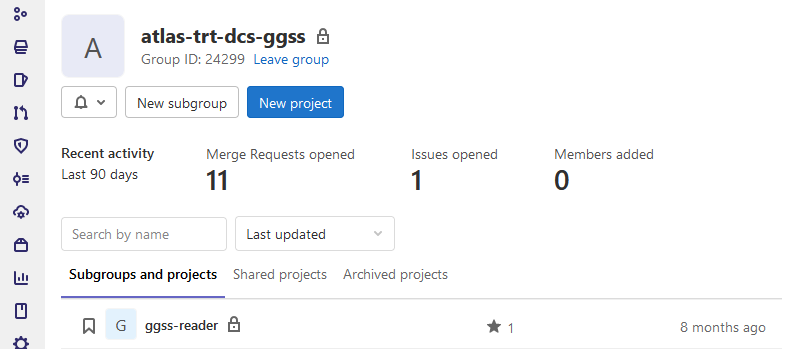
\includegraphics[width=\textwidth]{gitlab}
    \caption{Panel grupy \emph{atlas-trt-dcs-ggss} utworzonej na platformie GitLab.}
    \label{fig:gitlab}
\end{figure}

Omawiany portal wzbogaca ponadto współpracę opartą na repozytoriach poprzez wprowadzenie tzw. \emph{merge request}. Pozwalają one na współpracę przy łączeniu dwóch gałęzi repozytorium w~jedno. Rysunek \ref{fig:merge} przedstawia część przykładowego panelu \emph{merge request}. Oprócz logu wydarzeń widoczne są informację na temat: osoby, która zatwierdziła zmiany, statusu skonfigurowanej automatyzacji, czy też stanu danego \emph{merge request}. Dostępne są również zakładki, gdzie przeglądać można wszystkie rewizje wchodzące w~skład dołączanej gałęzi oraz wprowadzone w~ich ramach zmiany.

\begin{figure}[H]
    \centering
    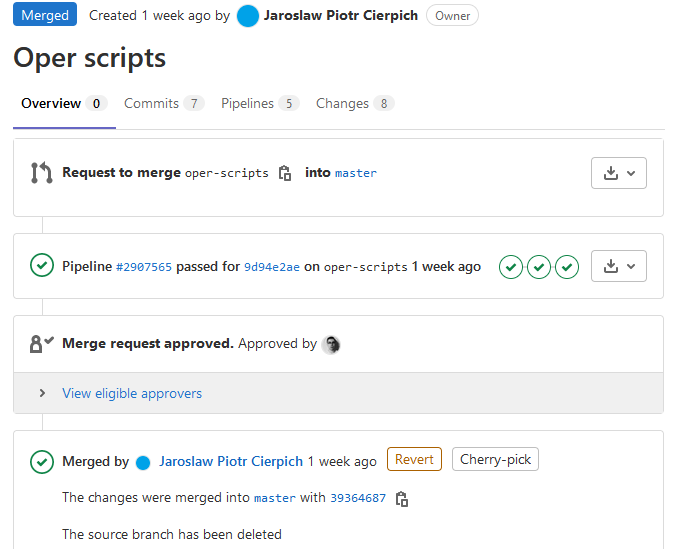
\includegraphics[width=\textwidth]{gitlab_merge}
    \caption{Przykładowy \emph{merge request} na platformie GitLab.}
    \label{fig:merge}
\end{figure}

Wraz ze wzrostem popularności portali takich jak GitLab zaczęto wprowadzać dodatkowe udogodnienia dla programistów, skupione szczególnie na procesie wytwarzania kodu, infrastrukturze do tego stosowanej oraz różnym praktykom stosowanym w~nowoczesnych projektach. Jedną z~takich funkcjonalności jest GitLab CI/CD, czyli część portalu GitLab oraz platforma pozwalająca na automatyzację procesu wytwórczego poprzez zastosowanie podejścia Continuous Integration/Continuous Delivery. GitLab CI/CD pozwala na zdefiniowanie akcji, które mają być wykonywane automatycznie w~przypadku wystąpienia pewnych zdarzeń, np: automatyczne wykonanie testów w~momencie umieszczenia nowej rewizji na portalu GitLab, czy też utworzenie nowego wydania aplikacji po przekazaniu odpowiedniej etykiety (ang. \emph{tag}) do repozytorium na platformie.

Wszystkie akcje zawarte w~ramach wyżej opisanej automatyzacji wykonywane są na specjalnie przygotowanych maszynach wirtualnych zarejestrowanych w~portalu GitLab, czyli tzw. \emph{GitLab Runners}. Maszyny te posiadają zainstalowane odpowiednie rozszerzenia oraz oprogramowanie Docker \cite{docker_main}, ponieważ większość akcji wykonywana jest w~ramach kontenerów.


\section{Narzędzie CMake (AK)}
CMake jest rozwijanym przez firmę \emph{Kitware} narzędziem automatyzującym procesy związane z~cyklem życia oprogramowania, w~tym przede wszystkim jego budowanie, testowanie, instalację oraz tworzenie pakietów. Udostępnia intuicyjny, oparty o~prosty język skryptowy interfejs, umożliwiający tworzenie konfiguracji w~sposób niezależny od docelowej platformy, dzięki czemu możliwe jest konstruowanie zaawansowanych, dostosowanych do potrzeb konkretnego projektu systemów budowania. Stanowi trzon systemu budowania i~pakietowania przygotowanego na potrzeby systemu GGSS przez autorów niniejszego manuskryptu w~ramach napisanej przez nich pracy inżynierskiej. Z~narzędziem CMake ściśle zintegrowane są systemy CPack oraz CTest, który zadaniem jest kolejno: tworzenie pakietów instalacyjnych z~oprogramowaniem (np. \lstinline{.rpm}) oraz tworzenie konfiguracji umożliwiających testowanie automatyczne.

Na listingu \ref{lst:cmake_example} przedstawiony został bardzo prosty przykład pliku \lstinline{CMakeLists.txt}, zawierającego konfigurację pozwalająca na zbudowanie aplikacji napisanej w~języku C++. Na załączonym fragmencie kodu widoczne są komendy pozwalające określić informacje takie jak: minimalna wersja narzędzia CMake, nazwa oraz wersja projektu czy lista plików wchodzących w~skład tworzonej aplikacji.

\lstinputlisting[
    language=CMake, 
    caption={Przykład pliku \lstinline{CMakeLists.txt}, zawierającego komendy pozwalające na zbudowanie prostej, składającej się z~jednego pliku źródłowego, aplikacji napisanej w~języku C++}, 
    label={lst:cmake_example}
]{2_technologies/code_samples/cmake_example.cmake}

\section{Menadżer pakietów RPM (JC)}
\emph{RPM Package Manager} \cite{rpm} \cite{rpm_wiki} jest systemem do zarządzania pakietami na systemach z~rodziny Red Hat, Fedora, CentOS, OpenSUSE. Posługuje się on pakietami z~rozszerzeniem \lstinline{.rpm}. W~ramach takiego pakietu zawarte są:
\begin{itemize}
    \item główna zawartość, np. skompilowana aplikacja czy gotowy skrypt powłoki Bash \cite{bash}
    \item metadane: informacje o~autorze, zawartości, wersji zawartości, opis pakietu, wymagane zależności
    \item logika instalacji oraz logika dezinstalacji: skrypty mające na celu przygotowanie systemu do instalacji oraz posprzątanie systemu po dezinstalacji pakietu
\end{itemize}

Instalacja oprogramowania za pomocą menadżera pakietów pozwala na znaczne przyspieszenie procesu. Zazwyczaj wszystkie akcje, które są wymagane przed zainstalowaniem oprogramowania, wykonywane są w~ramach logiki instalacji. Menadżer pakietów, wykorzystując zewnętrzne repozytoria, jest w~stanie pobrać i~zainstalować wszystkie wymagane przez instalowany pakiet zależności. Dodatkowo menadżer pakietów RPM zapewnia weryfikacje poprawności pakietu w~postaci technologii GPG oraz MD5.

